So far we have focused our work on the reliability and quality of the bluetooth data transferring. It is a well-known fact that the Lego brick is affected of a delay problems and this makes difficult to receive good data from it. \\ We solved the problem by making the data buffer unidirectional; in other words once our program has been started it stars to send the data to the pc. \\This permits:  

\begin{itemize}
\item a very high reading frequency: (500 hz),
\item high reliability, since the code is integrated directly into the system developed by Michele Bianchi, 
\item a control over the data flow, that permits to manage the inconsistent and redundancy data. 
\end{itemize}

Our program need of the following components in order to work: 
\begin{itemize}
\item LEGO MINDSTORMS NXT Brick;
\item LEGO MINDSTORMS NXT Interactive Motor;
\item Our software, included into the brofist directory;
\end{itemize}
In particular the LEGO MINDSTORMS is an interactive motor what works a 9V with internal gears (overall gear ratio 1:48) that has also an embedded rotation encoder with a resolution of 1?.
\begin{figure} [htb!]
  \centering
 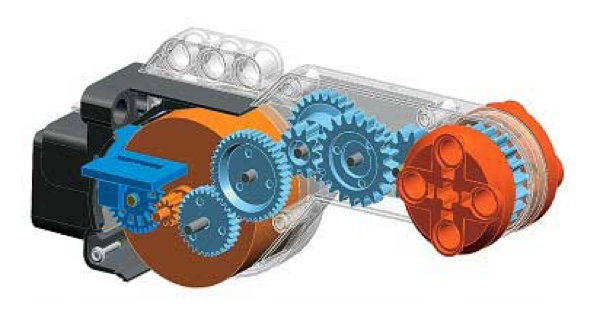
\includegraphics[scale = 0.40]{Graphics/legomotor.png}
 \caption{Picture 1.1. The Lego Motor}
  \label{fig:pos} 
\end{figure}
From this motor it is possible to set two kind of data: 
\begin{itemize}
\item Servo Motor revolution count in degree, by setting a positive or negative value it is possible to make the motor run either in a clockwise or not way.
\item Servo Motor PWM value and brake mode, this value regards the velocity percentage of the motor (if set to zero stops it); 
\end{itemize}

